Nesta seção, são apresentadas as equações utilizadas para o dimensionamento geométrico dos elementos de fundação, que fundamentam  a formulação das funções
de restrição empregadas no processo de otimização (ver Seção \ref{sec:method}). Tais equações visam assegurar o atendimento aos critérios técnicos e normativos brasileiros estabelecidos pela NBR 6118 \cite{nbr6118} e pela NBR 6122 \cite{nbr6122}.

\subsection{Tensão normais no solo}

A tensão resistente, ou tensão admissível do solo ($\sigma_{adm}$), é definida em função das características geotécnicas do terreno, sendo dependente principalmente do tipo de solo. Na prática, é comum a adoção de correlações empíricas baseadas no índice de resistência à penetração obtido por meio do ensaio SPT (\textit{Standard Penetration Test}), amplamente empregado em investigações geotécnicas no Brasil. 
Nesse contexto, as Equações \eqref{eq:tensão_rd_silte} a \eqref{eq:tensão_rd_pedregulho} apresentam as expressões adotadas neste trabalho para determinar a tensão admissível do solo em função do tipo de material identificado:

\begin{equation}
\sigma_{\text{adm}} = \frac{ N_{spt}}{50} \cdot 1000  \qquad \; \text{Silte ou argila{}},
\label{eq:tensão_rd_silte}
\end{equation}

\begin{equation}
\sigma_{\text{adm}} = \frac{ N_{spt}}{40} \cdot 1000  \qquad \; \text{Areia{}},
\label{eq:tensão_rd_areia}
\end{equation}

\begin{equation}
\sigma_{\text{adm}} = \frac{ N_{spt}}{30} \cdot 1000  \qquad \; \text{Pedregulho{}}.
\label{eq:tensão_rd_pedregulho}
\end{equation}

Nessas expressões, $N_{spt}$\footnote{$N_{\text{spt}}$: Numero de golpes obtido no ensaio $SPT$ ($Standard\; Penetration \; Test$) para cravar os últimos 30 cm do amostrador para cada metro de sondagem. Valores tipicamente entre 2 e 40 para solos argilosos e siltosos. Fórmula válida para $N_{\text{spt}} \leq 20$.} é o valor obtido no ensaio $SPT$ ($Standard\; Penetration \; Test$) o coeficiente multiplicativo de 1000 é utilizado para a conversão da tensão admissível para a unidade de quilopascal ($kPa$).

A tensão de na sapata é calculada em função da tensão causada pelo esforço vertical ($\sigma_{Fz}$), e pelos momentos fletores, em módulo, atuantes nas direções $x$ e $y$ ($M_{xk}$ e $M_{yk}$), conforme as  Equações \eqref{eq:sigma_max} e \eqref{eq:sigma_min}:

\begin{equation}
\sigma_{\text{max}} = \sigma_{Fz} \cdot \left( 1 + \frac{6 \cdot | M_{xk} |}{F_{zk} \cdot h_x} + \frac{6 \cdot |M_{yk}|}{F_{zk} \cdot h_y} \right),
\label{eq:sigma_max}
\end{equation}

\begin{equation}
\sigma_{\text{min}} = \sigma_{Fz} \cdot \left( 1 - \frac{6 \cdot | M_{xk}|}{F_{zk} \cdot h_x} - \frac{6 \cdot |M_{yk}|}{F_{zk} \cdot h_y} \right).
\label{eq:sigma_min}
\end{equation}

A tensão vertical $\sigma_{Fz}$ é definida pela Equação \eqref{eq:sigma_fz}, onde o coeficiente 1,05 refere-se ao acréscimo de tensão para corresponder ao peso próprio do elemento estrutural (ABNT, \citeyear{nbr6122}). As variáveis $h_x$ e $h_y$ são, respectivamente, as dimensões da sapata em $x$ e $y$. Os esforços $F_{zk}$, $M_{xk}$ e $M_{yk}$ são provenientes da superestrutura e são transferidos aos elementos de fundação por meio dos pilares. O fator 6 é uma constante geométrica que surge do módulo de resistência elástico de uma seção retangular. 
 
\begin{equation}
    \sigma_{Fz} = \frac{1,05 \cdot F_{zk}}{h_x \cdot h_y}.
    \label{eq:sigma_fz}
\end{equation}

A determinação da tensão atuante em cada sapata, necessita-se considerar todas as combinações de esforços provenientes da superestrutura. A partir dessas combinações, identifica-se aquela que resulta na condição mais desfavorável de solicitação, a qual será utilizada no dimensionamento da fundação.

Para garantir a viabilidade técnica da solução de fundação, as tensões solicitantes devem ser inferiores à tensão admissível do solo, atendendo aos critérios normativos de segurança e desempenho. Para as tensões de compressão (positivas), aplica-se um coeficiente de ponderação de 1,30 para a obtenção da tensão de cálculo. Já para as tensões de tração (negativas), adota-se o fator 1,00, uma vez que esforços de tração não são admitidos na interface solo-fundação.
\subsection{Projeto geométrico} 

A verificação geométrica consiste na imposição de uma restrição dimensional mínima entre a sapata e o pilar. Para cada direção principal $x$ e $y$, neste trabalho, exige-se que a dimensão da sapata seja superior à dimensão correspondente do pilar, acrescida de uma folga $\delta$ de cada lado, conforme as Equações \eqref{eq:folga_x} e \eqref{eq:folga_y}:

\begin{equation}
    h_x \ge a_p + 2 \cdot\delta,
    \label{eq:folga_x}
\end{equation}

\begin{equation}
    h_y \ge b_p + 2 \cdot \delta,
    \label{eq:folga_y}
\end{equation}

em que $h_x$ e $h_y$ representam as dimensões da sapata em planta, enquanto $a_p$ e $b_p$ correspondem às dimensões do pilar.

% \begin{equation}
%  \dfrac{h_z}{2} \leq C_x \leq 2 \cdot h_z
%      \label{eq:CEB-70 para direção x}
% \end{equation}

% \begin{equation}
%  \dfrac{h_z}{2} \leq C_y \leq 2 \cdot h_z
%      \label{eq:CEB-70 para direção y}
% \end{equation}


% O cálculo dos balanços nas direções $x$ e $y$ ($C_x$ e $C_y$) são determinados pelas Equações \eqref{eq:balanço_x} e \eqref{eq:balanço_y}

% \begin{equation}
%  C_x = \frac{h_x - a_p}{2}
%      \label{eq:balanço_x}
% \end{equation}

% \begin{equation}
%  C_x = \frac{h_y - b_p}{2}
%      \label{eq:balanço_y}
% \end{equation}

% Onde $h_x$ e $h_y$ são as dimensões em $x$ e $y$ da sapata. $a_p$ e $b_p$ são as dimensões do pilar em $x$ e $y$.

\subsection{Sobreposição de fundações}
\label{subsec:projeto_sobreposicao}

É essencial garantir que as sapatas não se sobreponham entre si, uma vez que a sobreposição inviabilizaria a execução e o desempenho estrutural, exigindo alternativas como sapatas associadas (que não são contempladas neste trabalho) ou reorganização dos elementos de fundação.
Para evitar a ocorrência de sobreposição geométrica do arranjo de fundações, é considerada uma verificação de sobreposição entre as sapatas, modeladas como retângulos alinhados aos eixos cartesianos. Ocorre sobreposição quando duas sapatas ocupam a mesma posição no plano, tal como apresentado na Figura \ref{fig:sobreposição}.

\begin{figure}[H]
    \centering
    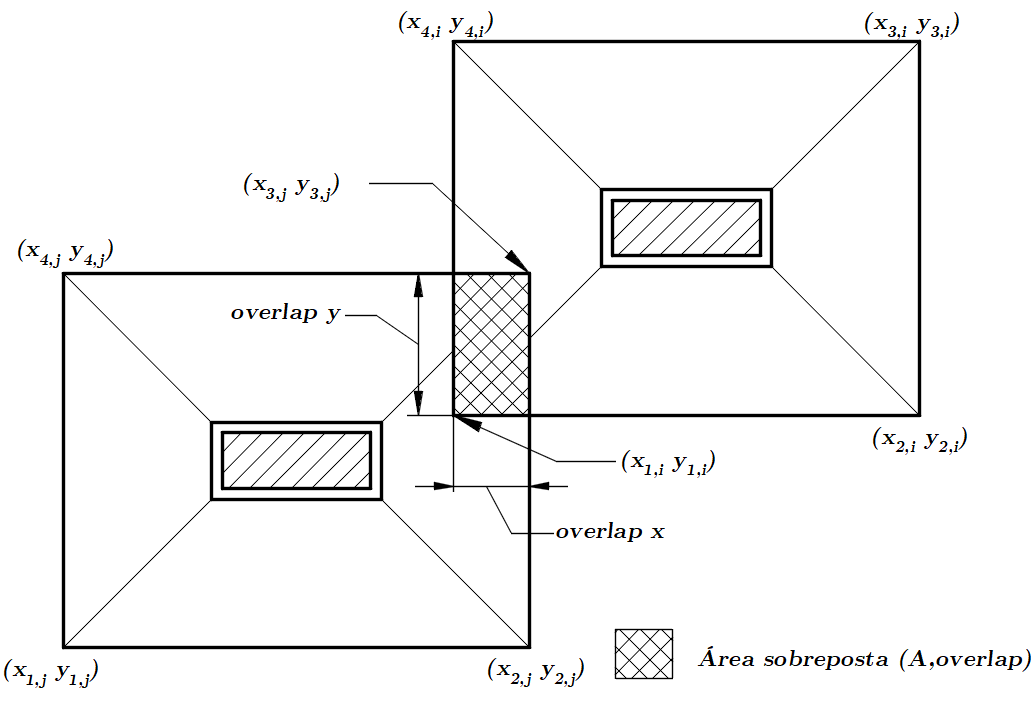
\includegraphics[width=0.9\linewidth]{figuras/sobreposição.png}
    \caption{Área de sobreposição entre duas sapatas.}
    \label{fig:sobreposição}
\end{figure}

Cada sapata é definida pelas coordenadas de seus vértices através das Equações \eqref{eq:coord_x1} a \eqref{eq:coord_y4}.
\begin{equation}
x_{1,i} = x_{g,i} - \frac{h_{x,i}}{2},
\label{eq:coord_x1}
\end{equation}

\begin{equation}
y_{1,i} = y_{g,i} - \frac{h_{y,i}}{2},
\label{eq:coord_y1}
\end{equation}

\begin{equation}
x_{2,i} = x_{g,i} + \frac{h_{x,i}}{2},
\label{eq:coord_x2}
\end{equation}

\begin{equation}
y_{2,i} = y_{g,i} - \frac{h_{y,i}}{2},
\label{eq:coord_y2}
\end{equation}

\begin{equation}
x_{3,i} = x_{g,i} + \frac{h_{x,i}}{2},
\label{eq:coord_x3}
\end{equation}

\begin{equation}
y_{3,i} = y_{g,i} + \frac{h_{y,i}}{2},
\label{eq:coord_y3}
\end{equation}

\begin{equation}
x_{4,i} = x_{g,i} - \frac{h_{x,i}}{2},
\label{eq:coord_x4}
\end{equation}

\begin{equation}
y_{4,i} = y_{g,i} + \frac{h_{y,i}}{2}.
\label{eq:coord_y4}
\end{equation}

A partir da análise simultânea de dois elementos de sapatas, chamadas de $i$ e $j$, é possível identificar o comprimento de sobreposição, denominado $overlap$, para as direções $x$ e $y$, obtidos através das Equações \eqref{eq:overlap_x} e \eqref{eq:overlap_y}.

\begin{equation}
\text{overlap}_x = \max\left(0,\ \min(x_{i,\max},\, x_{j,\max}) - \max(x_{i,\min},\, x_{j,\min})\right),
\label{eq:overlap_x}
\end{equation}

\begin{equation}
\text{overlap}_y = \max\left(0,\ \min(y_{i,\max},\, y_{j,\max}) - \max(y_{i,\min},\, y_{j,\min})\right).
\label{eq:overlap_y}
\end{equation}

A área de sobreposição é obtida pelo produto dos comprimentos $overlap$, apresentado na Equação \eqref{eq:area_sobreposição}. Esse valor é utilizado na penalização de sobreposição.

\begin{equation}
    A_{overlap} = overlap_x \cdot overlap_y.
    \label{eq:area_sobreposição}
\end{equation}

\subsection{Punção}

A verificação da punção será realizada conforme prescrito pela NBR 6118 para elementos estruturais de concreto armado \cite{nbr6118}. Esse procedimento consiste na análise da resistência ao cisalhamento em superfícies críticas sucessivas, definidas no entorno da região de aplicação do carregamento do pilar.

O esforço de punção atua em dois perímetros críticos, designados por $C$ e $C'$, conforme ilustrado na Figura \ref{fig: perímetro_critico}. O perímetro $C$ corresponde ao contorno do pilar enquanto $C'$ indica a região crítica localizada a uma distância de $2d$ da borda do pilar, sendo $d$ a altura útil da sapata.

\begin{figure}[htbp!]
    \centering
    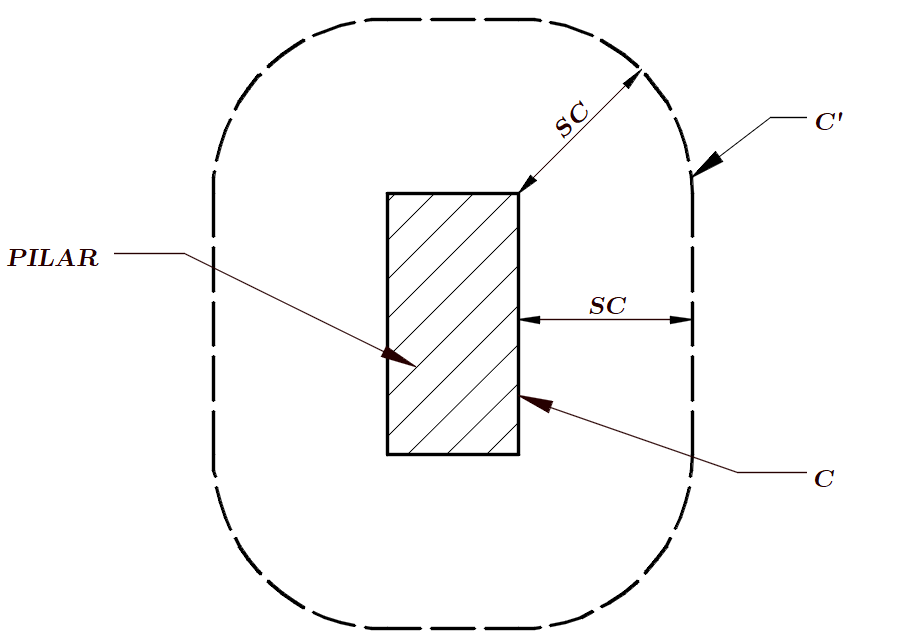
\includegraphics[width=0.5\linewidth]{figuras/perímetro_crítico.png}
    \caption{Perímetro crítico}
    \label{fig: perímetro_critico}
\end{figure}

A resistência da seção $C$ é determinada pela Equação~\eqref{eq:Tensão_resistente_C}

\begin{equation}
 \tau_{rd2} = 0,27 \cdot f_{cd} \cdot \alpha_{v2},
     \label{eq:Tensão_resistente_C}
\end{equation}

em que $f_{cd}$, a resistência de cálculo do concreto, é dado pela Equação \eqref{eq:fcd}

\begin{equation}
    f_{cd} = \frac{f_{ck}}{1,40},
        \label{eq:fcd}
\end{equation}

$\alpha_{v2}$ é definido pela Equação \eqref{eq:alpha_v2}, utilizando o valor de $f_{ck}$ em $MPa$

\begin{equation}
    \alpha_{v2} =  1 - \frac{f_{ck}}{250}.
        \label{eq:alpha_v2}
\end{equation}

 O cálculo da tensão solicitante de cálculo é dada pela Equação~\eqref{eq:Tensão_solicitante_C}.

\begin{equation}
 \tau_{sd2} = \frac{F_{zk} \cdot 1.4}{2 \cdot (a_p + b_p) \cdot d},
     \label{eq:Tensão_solicitante_C}
\end{equation}


em que $d$ é a altura útil, obtida pela Equação \eqref{eq:altura_util}, onde $cob$ indica o cobrimento mínimo da armadura.

\begin{equation}
    d = h_z - cob.
    \label{eq:altura_util}
\end{equation}


% O esforço de punção atua em dois perímetros críticos, designados por $C$ e $C'$, conforme ilustrado na figura. O perímetro $C$ corresponde ao contorno do pilar enquanto $C'$ indica a região crítica localizada a uma distância de $2d$ da borda do pilar, sendo $d$ a altura útil da sapata. Contudo a distância do perímetro $c'$, denominada na imagem como $SC$, será adotada a partir da expressão comumente utilizada de metade do $h_z$. 


% A verificação de punção consiste em definir a tensão solicitante ($\tau_{sd}$) e resistente ($\tau_{rd}$) para os dois perímetros. Assim sendo, para o perímetro $C$ tem-se os cálculos seguintes: Primeiramente, é definida a altura útil, Equação \eqref{eq:altura_util}. Em seguida, é determinada a tensão solicitante  no perímetro $C$ $\tau_{sd2}$ pela 


% Sendo $a_p$ e $b_p$ as dimensões do pilar em metros, nas direções de $x$ e $y$, respectivamente. $h_z$ é a altura do elemento de fundação em metros e $cob$ a espessura do cobrimento da armadura em metros. $f_{ck}$ e $f_{cd}$ são, respectivamente, a resistência característica e de cálculo do concreto em $MPa$.
% Em seguida, deve-se calcular a tensão resistente  no perímetro $C$ $\tau_{rd2}$, dada pela Equação \eqref{eq:Tensão_resistente_C}:



% No perímetro $C'$, a tensão resistente $\tau_{rd2}$ é dada pela Equação \eqref{eq:Tensão_resistente_C'}:

% \begin{equation}
%  \tau_{rd1} = 0,13 \cdot k_e \cdot \left( 100 \cdot \rho \cdot f_{ck} \right) ^\frac{1}{3}  + 0,1 \cdot \sigma_{cp}
%      \label{eq:Tensão_resistente_C'}
% \end{equation}

% Onde $k_e$ é o coeficiente de escala de punção identificado pela Equação \eqref{eq:ke}, $\rho$ é a taxa geométrica de armadura de flexão aderente, definida pela tabela ?????. $\sigma_{sp}$ é a tensão devida a ação de elementos protendidos.

% \begin{equation}
% k_e = 1 + \sqrt{\frac{20}{d \cdot 100}}
% \label{eq:ke}
% \end{equation}

% A tensão solicitante no perímetro $C'$ é dada pela \eqref{eq:Tensão_solicitante_C'}:

% \begin{equation}
%  \tau_{sd1} = \frac{1,4 \cdot F_{zk}}{u \cdot d} + \frac{1,4 \cdot k_x \cdot M_{xk}}{w_{px} \cdot d} + \frac{1,4 \cdot k_y \cdot M_{yk}}{w_{py} \cdot d}
%      \label{eq:Tensão_solicitante_C'}
% \end{equation}

% Nesta equação, $k_x$ e $k_y$ referem-se a coeficientes que indicam a parcela de transmissão do momento ao pilar por cisalhamento. Estes são obtidos pela tabela 19.2 da NBR 6118. $w_{px}$ e $w_{py}$ são definidos pelas Equações \eqref{eq:wpx} e \eqref{eq:wpy}, respectivamente. $d$ é a altura útil definida anteriormente neste item. $u$ representa o perímetro crítico $C'$ dado pela Equação \eqref{eq:perímetro_c'}.

% \begin{equation}
% w_{px} = \frac{a_p^2}{2} + a_p \cdot b_p + 4 \cdot b_p \cdot sc + 16 \cdot sc^2 + 2 \cdot \pi \cdot a_p \cdot sc
% \label{eq:wpx}
% \end{equation}

% \begin{equation}
% w_{py} = \frac{b_p^2}{2} + b_p \cdot a_p + 4 \cdot a_p \cdot sc + 16 \cdot sc^2 + 2 \cdot \pi \cdot b_p \cdot sc
%     \label{eq:wpy}
% \end{equation}

% \begin{equation}
% u = 2 \cdot \left( a_p + b_p \right) + 4 \pi \cdot sc 
%     \label{eq:perímetro_c'}
% \end{equation}


% Em que $sc$ representa a distância da seção crítica da borda do pilar conforme a figura \eqref{fig: perímetro_critico}, dada pela Equação \eqref{eq:secao_critica}:
% %\begin{equation}
% %u_{rd2} = 2 \cdot (a_p + b_p)
%  %   \label{eq:urd2}
% %\end{equation}


% \begin{equation}
% sc = \frac{h_z}{2}
%     \label{eq:secao_critica}
% \end{equation}


% Após definidas as tensões solicitantes e resistentes, são feitas as verificações aprepresentadas no item 4 deste trabalho.

% As equações a seguir talvez devam ir para a metodologia, pois são utilizadas pelo código para "interpretar" tabelas da norma:

% \begin{equation}
% rho = \frac{\sqrt{rho_x * rho_y}}{100}
%     \label{eq:rho}
% \end{equation}

% \begin{equation}
% C1\_C2 = \frac{a_p}{b_p}
%     \label{eq:c1-C2}
% \end{equation}

% \begin{equation}
% C2\_C1 = \frac{b_p}{a_p}
%     \label{eq:C2-C1}
% \end{equation}
